\documentclass[12pt, twoside]{article}
\usepackage[letterpaper, margin=1in, headsep=0.5in]{geometry}
\usepackage[english]{babel}
\usepackage[utf8]{inputenc}
\usepackage{amsmath}
\usepackage{amsfonts}
\usepackage{amssymb}
\usepackage{tikz}
%\usetikzlibrary{quotes, angles}

\usepackage{graphicx}
\usepackage{enumitem}
\usepackage{multicol}

\usepackage{fancyhdr}
\pagestyle{fancy}
\fancyhf{}
\renewcommand{\headrulewidth}{0pt} % disable the underline of the header

\fancyhead[RE]{\thepage}
\fancyhead[RO]{\thepage \\ Name: \hspace{3cm}}
\fancyhead[L]{BECA / Dr. Huson / Geometry\\* 21 March 2019}

\begin{document}
\subsubsection*{8-13 Homework: Graphing inequalities algebra review}
For graphs, use a pencil and straight edge. Label each line.
  \begin{enumerate}

\item Solve for $y$, then graph the two inequalities.

  \begin{multicols}{2}
    $y > \frac{3}{4}x-5$ \\
    $2x+y \geq 6$
  \end{multicols}
  \vspace{2.5cm}

  \begin{center} %4 quadrant regents grid w T-Chart
  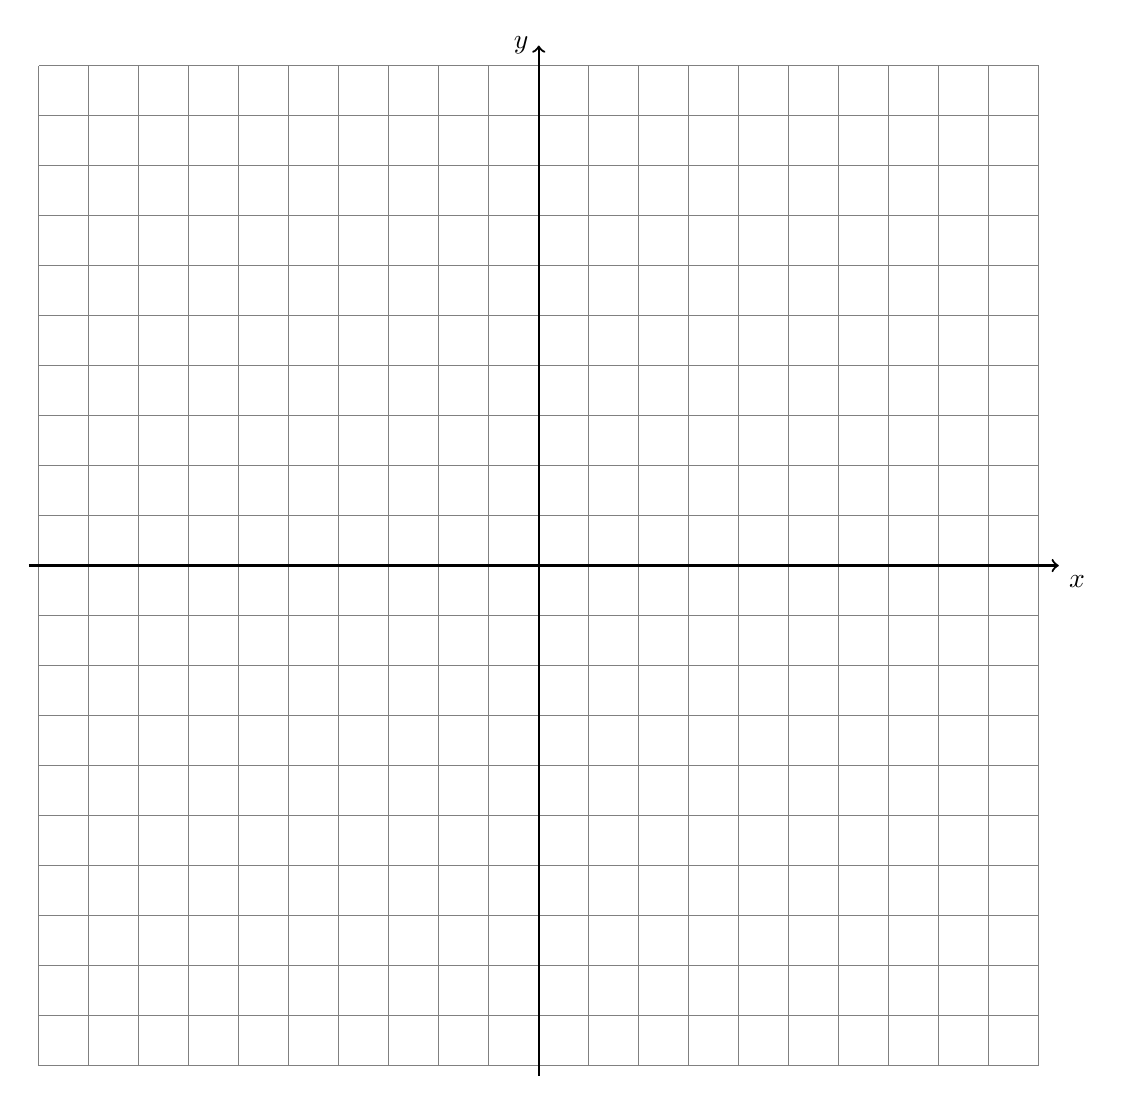
\begin{tikzpicture}[scale=.635]
    \draw [help lines] (-10,-10) grid (10,10);
    \draw [thick, ->] (-10.2,0) -- (10.4,0) node [below right] {$x$};
    \draw [thick, ->] (0,-10.2)--(0,10.4) node [left] {$y$};
  \end{tikzpicture}
  \end{center}

  Mark the solution set with a capital ``S". Is the point $(8,1)$ a solution? Justify your answer.
\newpage

\item Does the table represent a linear function? Justify your answer.
  \renewcommand{\arraystretch}{1.6}
    \begin{center}
      \begin{tabular}{|c|r|}
      \hline
      $x$ & $f(x)$\\
      \hline
      -1 & 3 \\
      \hline
      0 & 5 \\
      \hline
      1 & 0 \\
      \hline
      2 & 2 \\
      \hline
      3 & 4 \\
      \hline
      \end{tabular}
    \end{center}
 \vspace{2cm}
    \item Given $f(x)=-2x+11$. Simplify $f(3.5)$. \vspace{3cm}
    \item Find $g(x)=\frac{1}{3} x-2$ for $x=6$. \vspace{3.5cm}
    \item Given $\displaystyle h(x)=\frac{2x+3}{7}$. Evaluate the expression $h(-5)$. \vspace{4cm}


  \end{enumerate}
  \newpage
  \setcounter{page}{1}
  \subsubsection*{Skills Tracker: Graphing systems and inequalities}
  Use pencil for graph (1 point)
    \begin{enumerate}

    \item Solve for $y$, then graph the two lines. Label both lines and the solution to the system, the intersection, as a coordinate pair. (3 points)

      \begin{multicols}{2}
        $y = -3x -2$ \\
        $x-2y = -10$
      \end{multicols}
      \vspace{3cm}

      \begin{center} %4 quadrant regents grid w T-Chart
      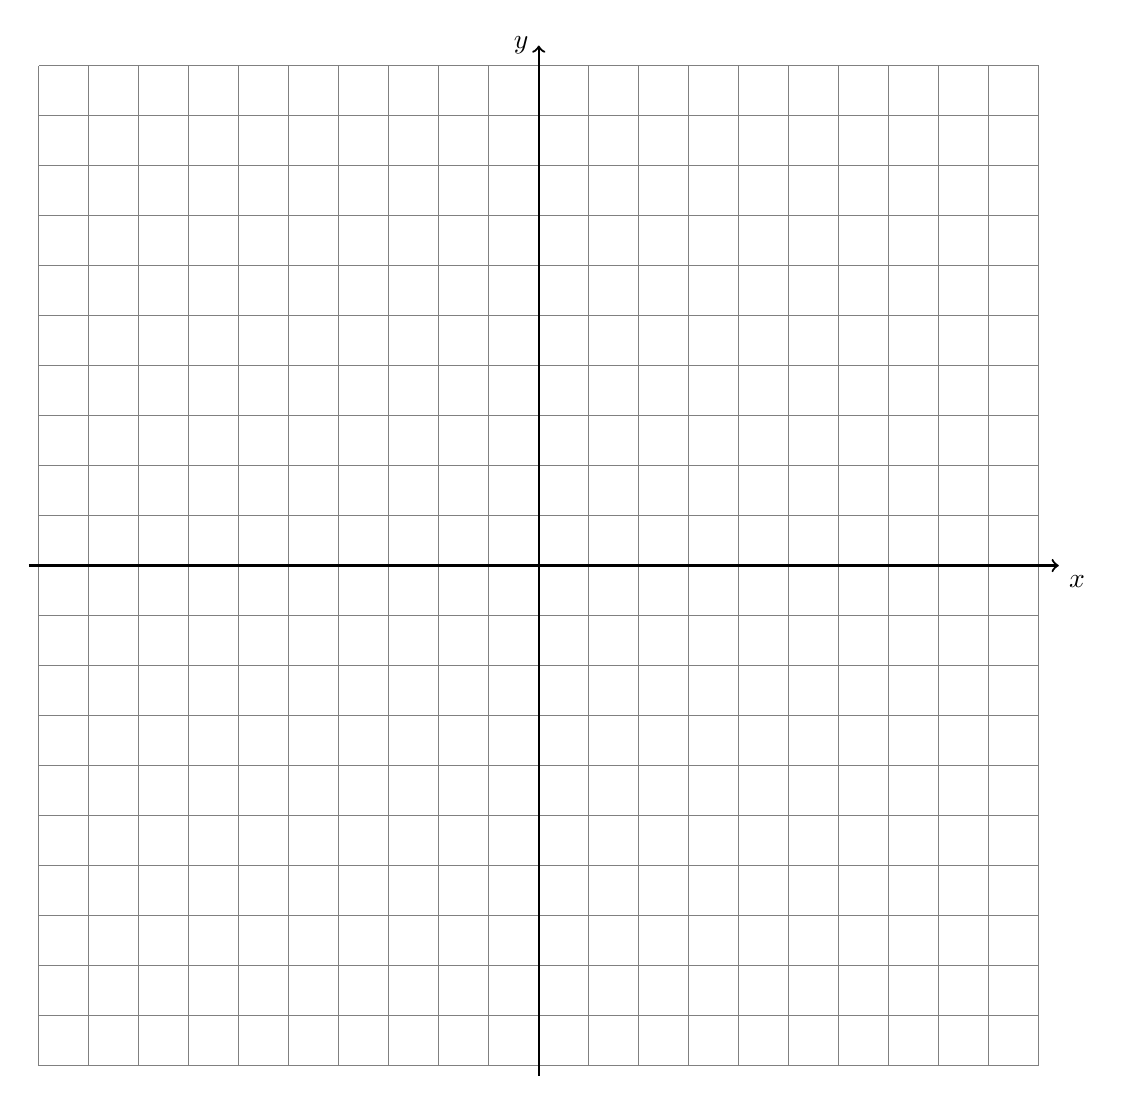
\begin{tikzpicture}[scale=.635]
        \draw [help lines] (-10,-10) grid (10,10);
        \draw [thick, ->] (-10.2,0) -- (10.4,0) node [below right] {$x$};
        \draw [thick, ->] (0,-10.2)--(0,10.4) node [left] {$y$};
      \end{tikzpicture}
      \end{center}

    \newpage
      \item Solve for $y$, then graph the two inequalities. Mark the solution set with a capital ``S."

        \begin{multicols}{2}
          $y < -\frac{2}{3}x+5$ \\
          $2x+y \geq -3$
        \end{multicols}
        \vspace{3cm}

        \begin{center} %4 quadrant regents grid w T-Chart
        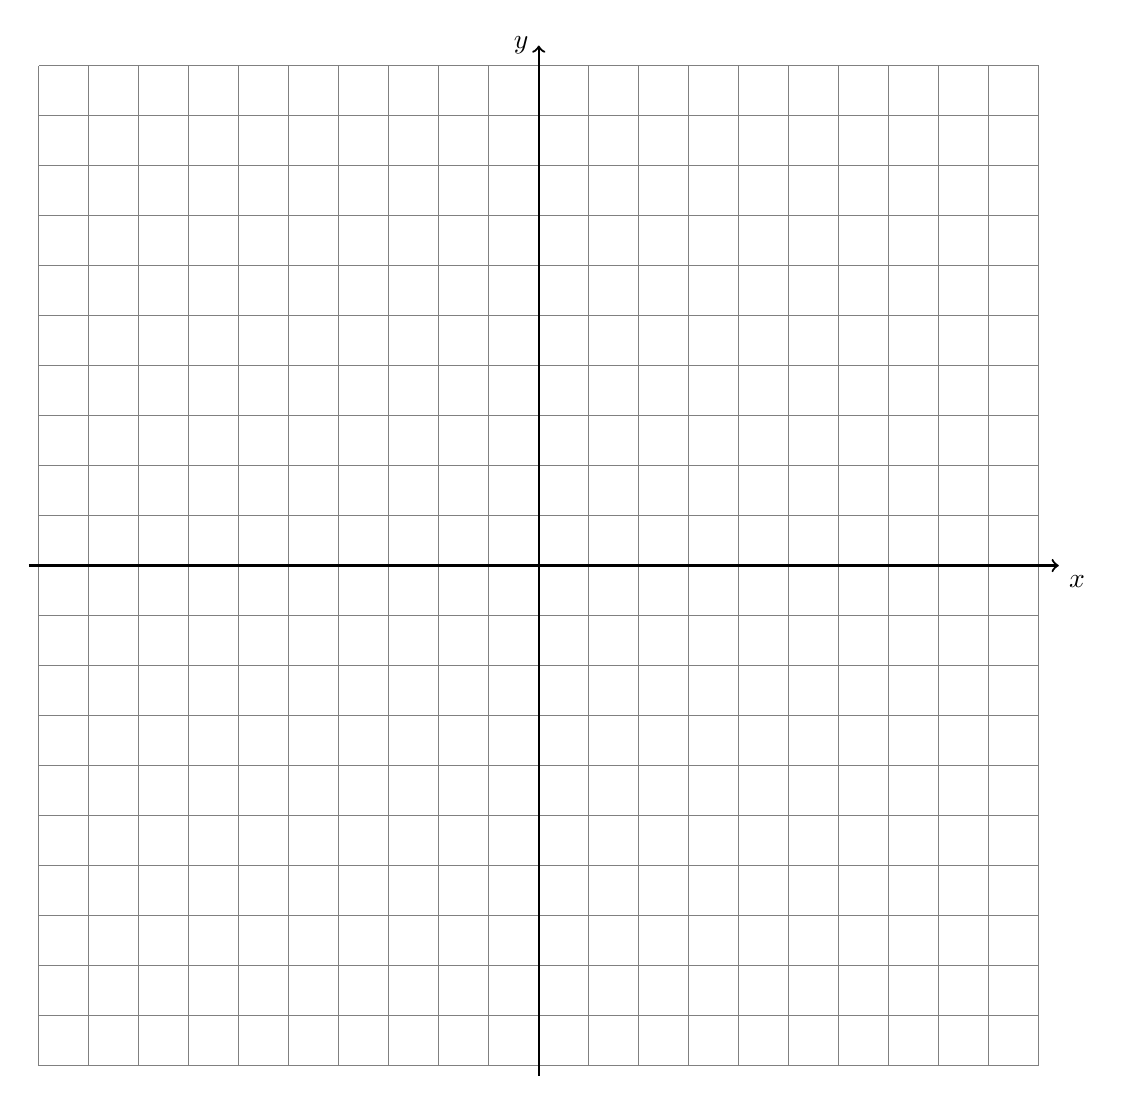
\begin{tikzpicture}[scale=.635]
          \draw [help lines] (-10,-10) grid (10,10);
          \draw [thick, ->] (-10.2,0) -- (10.4,0) node [below right] {$x$};
          \draw [thick, ->] (0,-10.2)--(0,10.4) node [left] {$y$};
        \end{tikzpicture}
        \end{center}
        Determine and state whether the point $(-4,1)$ is a solution of the system of inequalities. Justify your answer.



  \end{enumerate}
  \newpage
\subsubsection*{Do Now: Graphing inequalities}
Show your work. For graphs, {\large use a pencil and straight edge}. Graph the inequality after filling in the values in the blanks and circling the correct types.
  \begin{enumerate}

    \item $\displaystyle \frac{3}{2} x - 2y \leq  +2 $

        \vspace{0.25cm}
        \begin{multicols}{2}
          $y$-intercept $b= \rule{2cm}{0.15mm}$ \\[0.5cm]
          Slope \hspace{0.7cm} $m= \rule{2cm}{0.15mm}$\\[0.5cm]

          Line: \hspace{1cm} Solid ($=$) \hspace{0.45cm} Dashed ($\neq$)\\[0.5cm]
          Shading: \hspace{0.3cm} Above ($y>$) \hspace{0.25cm} Below ($y<$)\\
        \end{multicols}

    \begin{center} %4 quadrant regents grid w T-Chart
    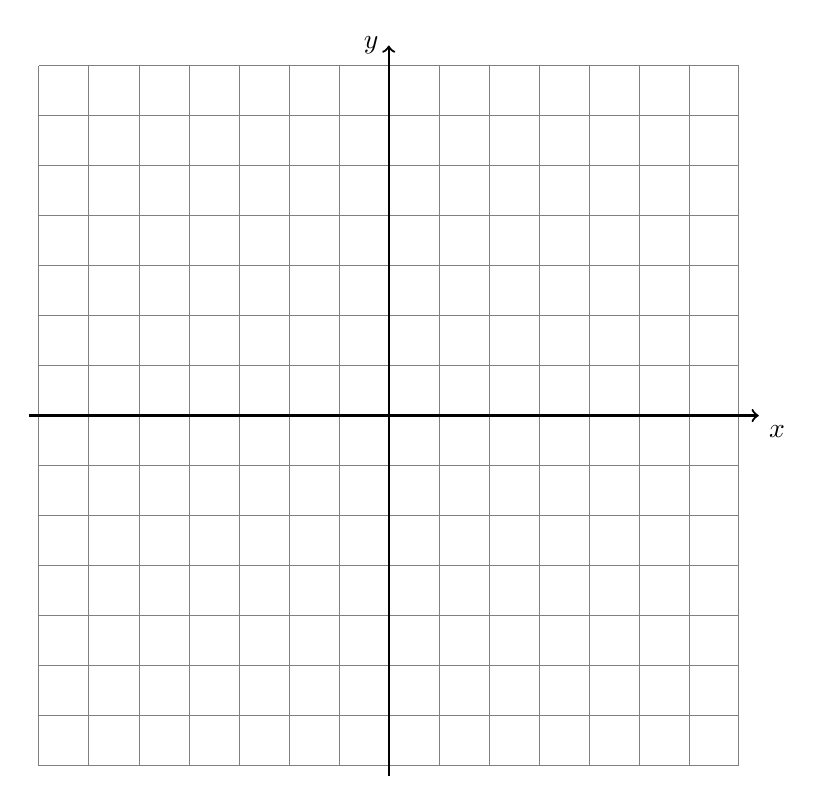
\begin{tikzpicture}[scale=.635]
      \draw [help lines] (-7,-7) grid (7,7);
      \draw [thick, ->] (-7.2,0) -- (7.4,0) node [below right] {$x$};
      \draw [thick, ->] (0,-7.2)--(0,7.4) node [left] {$y$};
    \end{tikzpicture}
    \end{center}

    \item Solve for $y$, then complete. $\displaystyle \frac{3}{2} x - 3y \geq 6 $

        \vspace{3cm}
        \begin{multicols}{2}
          \raggedcolumns
          $y$-intercept $b= \rule{2cm}{0.15mm}$ \\[0.5cm]
          Slope \hspace{0.7cm} $m= \rule{2cm}{0.15mm}$\\

          Line: \hspace{1cm} Solid ($=$) \hspace{0.45cm} Dashed ($\neq$)\\[0.5cm]
          Shading: \hspace{0.3cm} Above ($y>$) \hspace{0.25cm} Below ($y<$)
        \end{multicols}

    \newpage
    \item Graph the two inequalities after filling in the values in the blanks.\\[0.5cm]

      \begin{multicols}{2}
        $y \geq -3 x +1$ \\
        $y < -\frac{3}{2} x -2$
      \end{multicols}
      \begin{multicols}{2}
        \raggedcolumns
        \begin{enumerate}
          \item $y$-intercept $b= \rule{2cm}{0.15mm}$ \\[0.5cm]
          \item Slope \hspace{0.7cm} $m= \rule{2cm}{0.15mm}$\\[0.5cm]
        \end{enumerate}
        \begin{enumerate}
          \item $y$-intercept $b= \rule{2cm}{0.15mm}$ \\[0.5cm]
          \item Slope \hspace{0.7cm} $m= \rule{2cm}{0.15mm}$\\[0.5cm]
        \end{enumerate}
      \end{multicols}

      \begin{center} %4 quadrant regents grid w T-Chart
      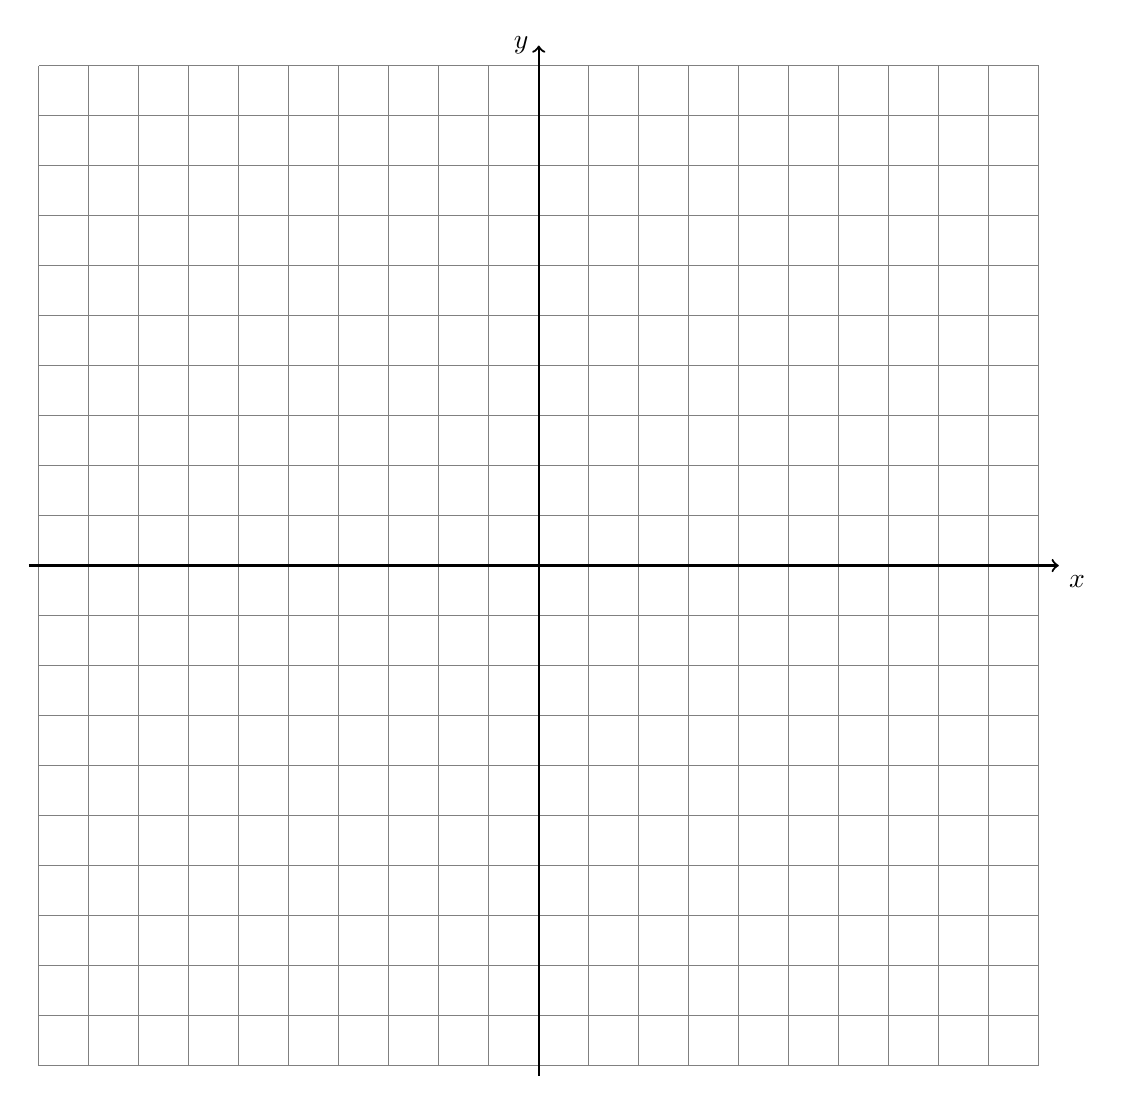
\begin{tikzpicture}[scale=.635]
        \draw [help lines] (-10,-10) grid (10,10);
        \draw [thick, ->] (-10.2,0) -- (10.4,0) node [below right] {$x$};
        \draw [thick, ->] (0,-10.2)--(0,10.4) node [left] {$y$};
      \end{tikzpicture}
      \end{center}

\newpage

\subsection*{Rate of change}

\item Find the slope of the function from the ratio of the line differences.

  \begin{multicols}{2}
  \begin{enumerate}
    \item
      \begin{tabular}{|c|r|}
      \hline
      $x$ & $f(x)$\\
      \hline
      -2 & -2 \\
      \hline
      -1 & 0 \\
      \hline
      0 & 2 \\
      \hline
      1 & 4 \\
      \hline
      2 & 6 \\
      \hline
      \end{tabular}\\[0.85cm]

      Change in $y$ $= \rule{2cm}{0.15mm}$ \\[0.5cm]
      Change in $x$ $= \rule{2cm}{0.15mm}$ \\[0.5cm]
      Slope $m= \rule{2cm}{0.15mm}$\\

    \item
      \begin{tabular}{|c|r|}
      \hline
      $x$ & $f(x)$\\
      \hline
      -4 & 9 \\
      \hline
      -2 & 6 \\
      \hline
      0 & 3 \\
      \hline
      2 & 0 \\
      \hline
      4 & -3 \\
      \hline
      \end{tabular}\\[0.85cm]

      Change in $y$ $= \rule{2cm}{0.15mm}$ \\[0.5cm]
      Change in $x$ $= \rule{2cm}{0.15mm}$ \\[0.5cm]
      Slope $m= \rule{2cm}{0.15mm}$\\


    \end{enumerate}
    \end{multicols}

  \item Find the slope of the function. If the rate of change is not constant, write, ``Non-linear. The rate of change is not constant."

    \begin{multicols}{2}
    \begin{enumerate}
      \item
        \begin{tabular}{|c|r|}
          \hline
          $x$ & $f(x)$\\
          \hline
          -3 & 0 \\
          \hline
          -1 & -2 \\
          \hline
          0 & -3 \\
          \hline
          1 & -4 \\
          \hline
          3 & -6 \\
          \hline
        \end{tabular}\\[0.85cm]

        Slope $m= \rule{2cm}{0.15mm}$\\


      \item
        \begin{tabular}{|c|r|}
          \hline
          $x$ & $f(x)$\\
          \hline
          -4 & 7 \\
          \hline
          -2 & 5 \\
          \hline
          0 & 3 \\
          \hline
          2 & 5 \\
          \hline
          4 & 7 \\
          \hline
        \end{tabular}\\[0.85cm]

        Slope $m= \rule{2cm}{0.15mm}$\\

      \end{enumerate}
    \end{multicols}

    \newpage
          \subsubsection*{Graphing quadratic functions}

          \item Given the quadratic function $f(x)=x^2-2$, find the row differences.
            \renewcommand{\arraystretch}{1.6}
              \begin{center}
                \begin{tabular}{|c|r|}
                \hline
                $x$ & $f(x)$\\
                \hline
                -3 & 7 \\
                \hline
                -2 & 2 \\
                \hline
                -1 & -1 \\
                \hline
                0 & -2 \\
                \hline
                1 & -1 \\
                \hline
                2 & 2 \\
                \hline
                3 & 7 \\
                \hline
                \end{tabular}
              \end{center}
          Graph the function as a line over the domain $-3 \leq x \leq 3$.

          \begin{center} %4 quadrant regents grid w T-Chart
          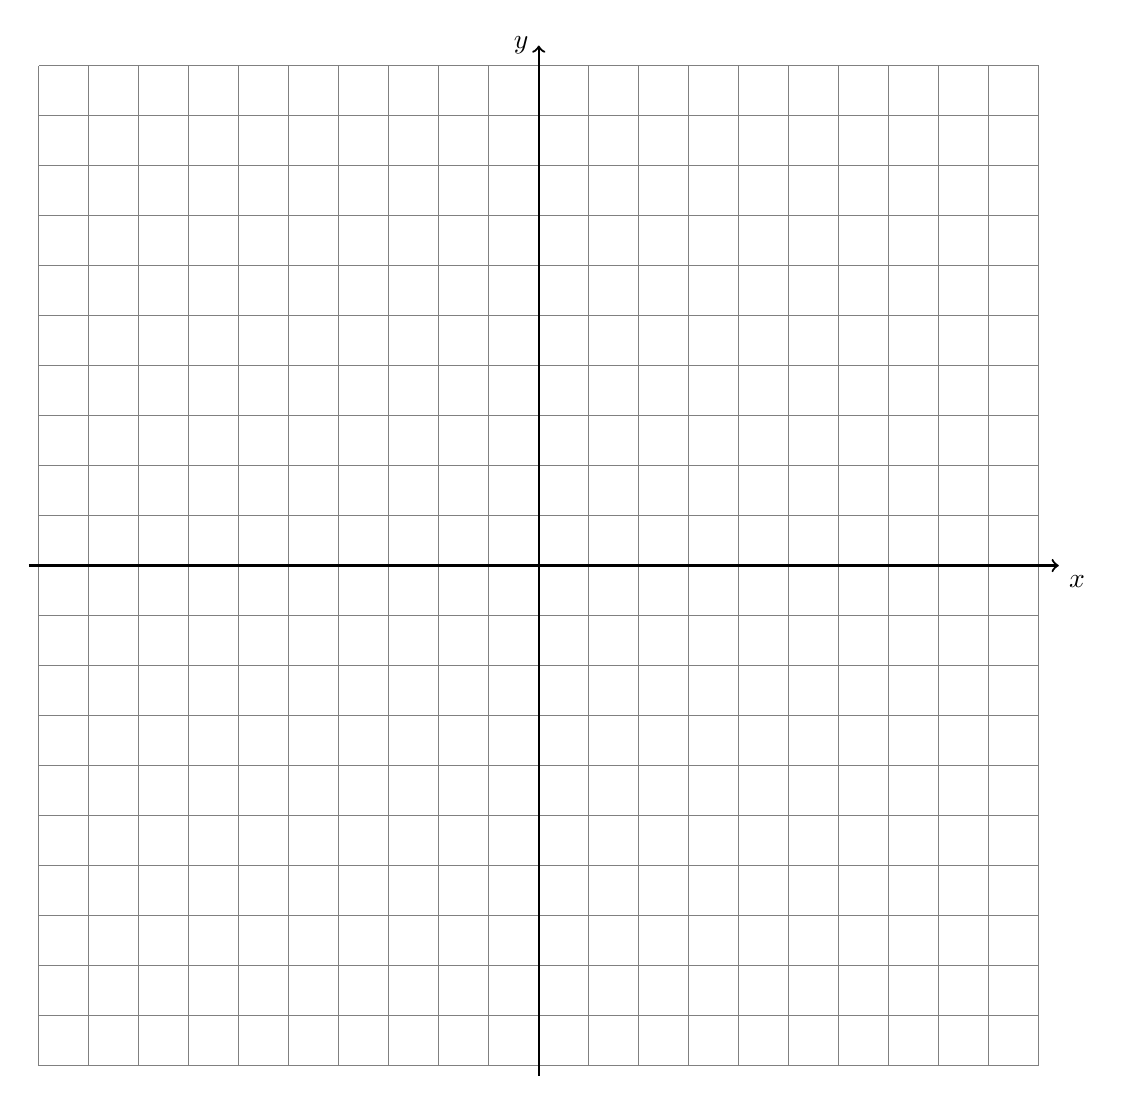
\begin{tikzpicture}[scale=.635]
            \draw [help lines] (-10,-10) grid (10,10);
            \draw [thick, ->] (-10.2,0) -- (10.4,0) node [below right] {$x$};
            \draw [thick, ->] (0,-10.2)--(0,10.4) node [left] {$y$};
          \end{tikzpicture}
          \end{center}


\end{enumerate}

\newpage
\setcounter{page}{1}
\subsubsection*{Homework: Graphing systems of equations}
\begin{enumerate}
    \item Graph the two lines after filling in the values in the blanks.\\[0.5cm]


    \begin{multicols}{2}
      $y> x -3$ \\
      $y \leq -\frac{1}{2} x +6$
    \end{multicols}
    \begin{multicols}{2}
      \raggedcolumns
      \begin{enumerate}
        \item $y$-intercept $b= \rule{2cm}{0.15mm}$ \\[0.5cm]
        \item Slope \hspace{0.7cm} $m= \rule{2cm}{0.15mm}$\\[0.5cm]
      \end{enumerate}
      \begin{enumerate}
        \item $y$-intercept $b= \rule{2cm}{0.15mm}$ \\[0.5cm]
        \item Slope \hspace{0.7cm} $m= \rule{2cm}{0.15mm}$\\[0.5cm]
      \end{enumerate}
    \end{multicols}

    Label both lines and the solution to the system with a capital "S". (3 points) Use pencil for graph (1 point)\\

    \begin{center} %4 quadrant regents grid w T-Chart
    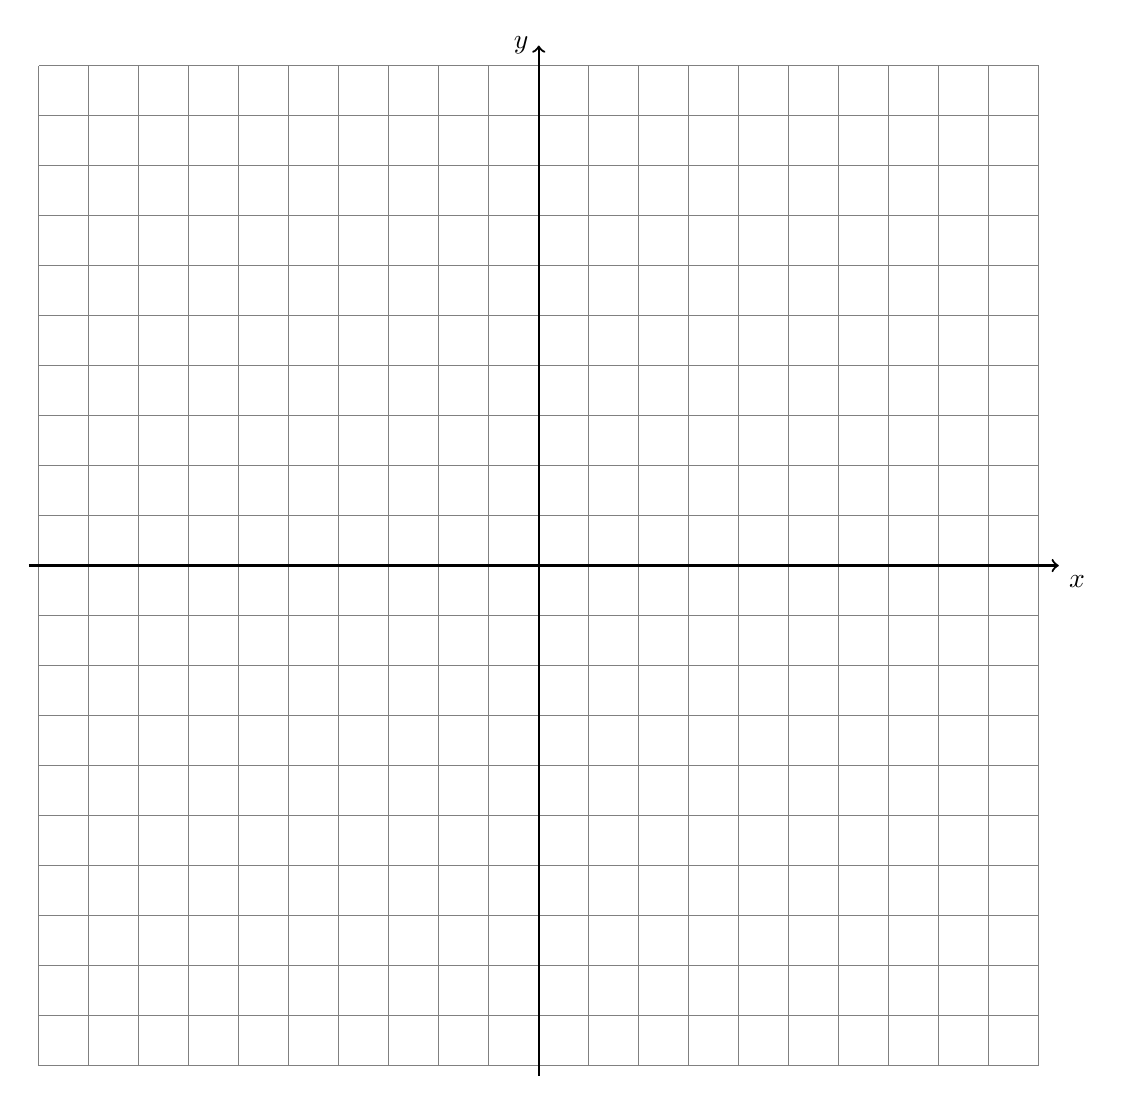
\begin{tikzpicture}[scale=.635]
      \draw [help lines] (-10,-10) grid (10,10);
      \draw [thick, ->] (-10.2,0) -- (10.4,0) node [below right] {$x$};
      \draw [thick, ->] (0,-10.2)--(0,10.4) node [left] {$y$};
    \end{tikzpicture}
    \end{center}

\end{enumerate}
\newpage
\setcounter{page}{1}
\subsubsection*{Classwork: Happy New Year!\\Due at the end of the period.}
Fill in the values in the blanks and circling the correct types.
  \begin{enumerate}

    \item $\displaystyle y \leq \frac{2}{3} x +1 $

      \vspace{0.25cm}
      \begin{multicols}{2}
        $y$-intercept $b= \rule{2cm}{0.15mm}$ \\[0.5cm]
        Slope \hspace{0.7cm} $m= \rule{2cm}{0.15mm}$\\[0.5cm]

        Line: \hspace{1cm} Solid ($=$) \hspace{0.5cm} Dashed ($\neq$)\\[0.5cm]
        Shading: \hspace{0.3cm} Above ($y>$) \hspace{0.25cm} Below ($y<$)\\
      \end{multicols}
      Graph the inequality (use a pencil and straight edge - 1 point)

      \begin{center} %4 quadrant regents grid w T-Chart
      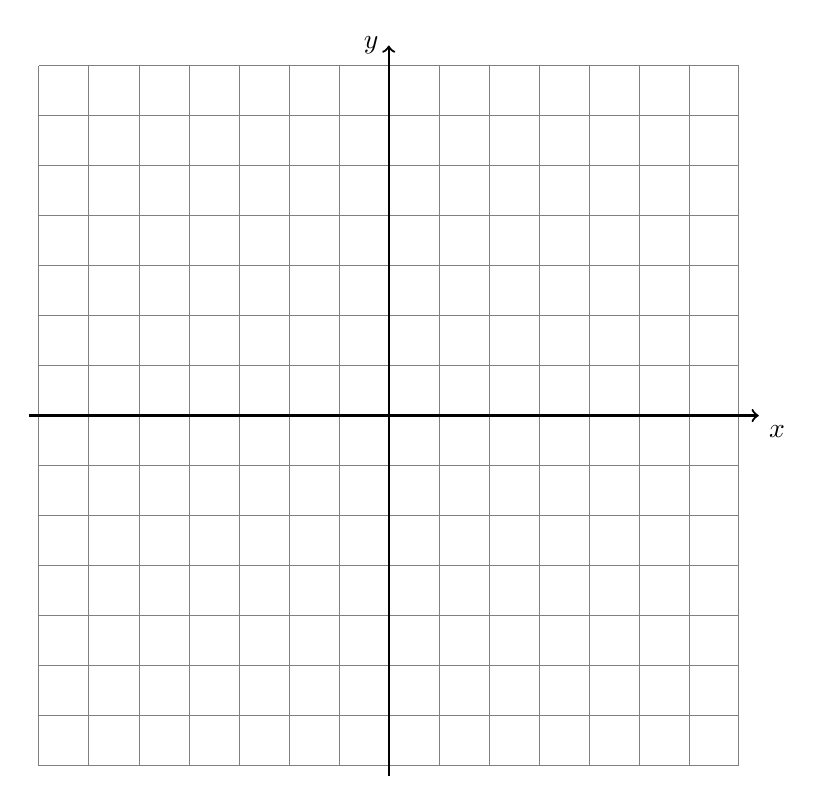
\begin{tikzpicture}[scale=.635]
        \draw [help lines] (-7,-7) grid (7,7);
        \draw [thick, ->] (-7.2,0) -- (7.4,0) node [below right] {$x$};
        \draw [thick, ->] (0,-7.2)--(0,7.4) node [left] {$y$};
      \end{tikzpicture}
      \end{center}

    \item Solve for $y$, then complete. $\displaystyle x+ 2y > 3 $

        \vspace{2cm}
        \begin{multicols}{2}
          \raggedcolumns
          $y$-intercept $b= \rule{2cm}{0.15mm}$ \\[0.5cm]
          Slope \hspace{0.7cm} $m= \rule{2cm}{0.15mm}$\\

          Line: \hspace{1cm} Solid ($=$) \hspace{0.5cm} Dashed ($\neq$)\\[0.5cm]
          Shading: \hspace{0.3cm} Above ($y>$) \hspace{0.25cm} Below ($y<$)
        \end{multicols}

    \newpage
    \item Graph the two lines after filling in the values in the blanks.\\[0.5cm]


    \begin{multicols}{2}
      $y= 2x -3$ \\
      $y=-\frac{1}{3} x +4 $
    \end{multicols}
    \begin{multicols}{2}
      \raggedcolumns
      \begin{enumerate}
        \item $y$-intercept $b= \rule{2cm}{0.15mm}$ \\[0.5cm]
        \item Slope \hspace{0.7cm} $m= \rule{2cm}{0.15mm}$\\[0.5cm]
      \end{enumerate}
      \begin{enumerate}
        \item $y$-intercept $b= \rule{2cm}{0.15mm}$ \\[0.5cm]
        \item Slope \hspace{0.7cm} $m= \rule{2cm}{0.15mm}$\\[0.5cm]
      \end{enumerate}
    \end{multicols}

    Label both lines and the solution to the system, the intersection, as a coordinate pair. (3 points) Use pencil for graph (1 point)\\

    \begin{center} %4 quadrant regents grid w T-Chart
    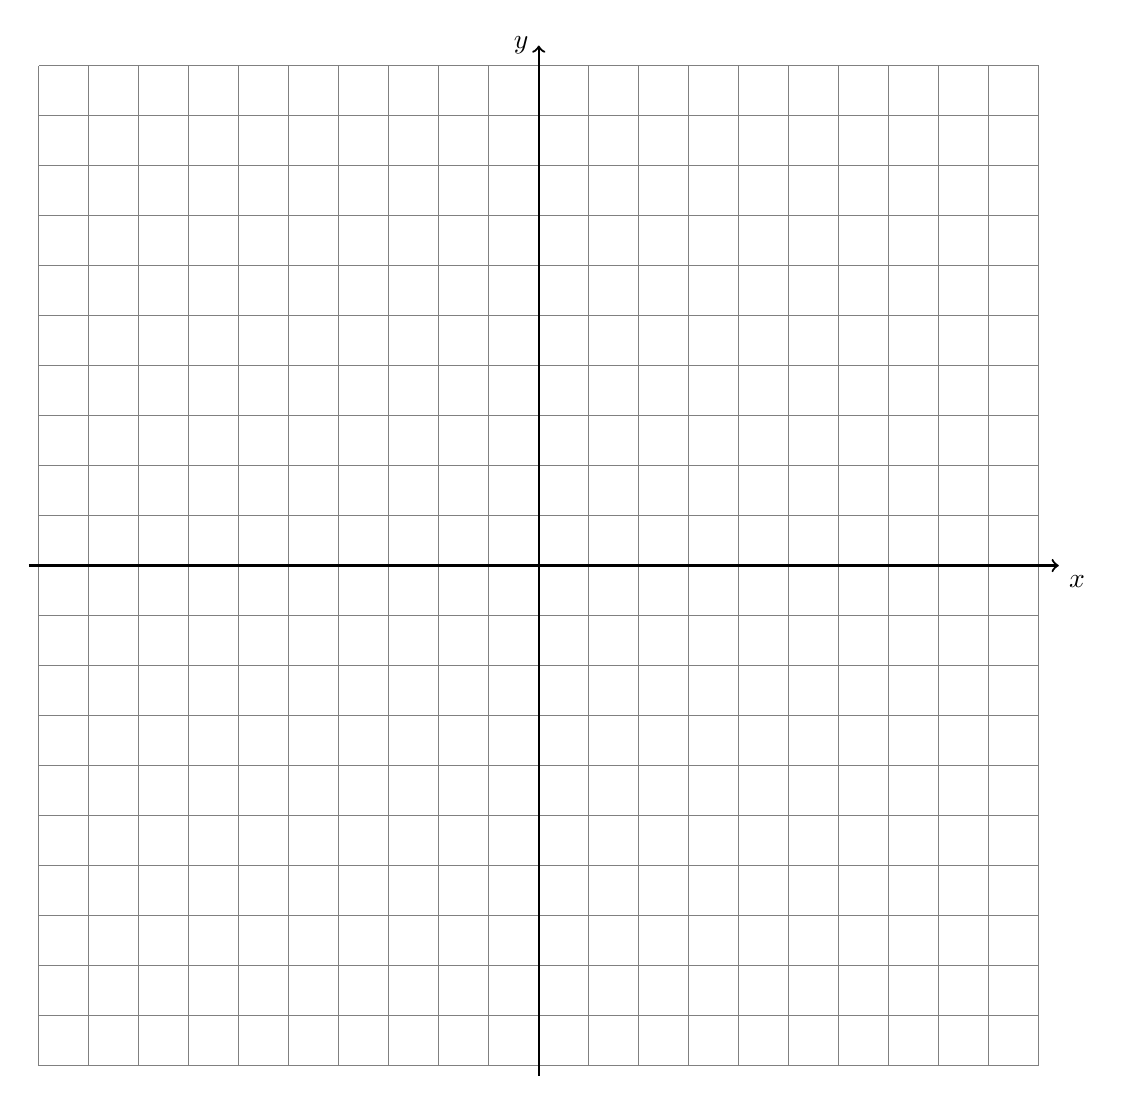
\begin{tikzpicture}[scale=.635]
      \draw [help lines] (-10,-10) grid (10,10);
      \draw [thick, ->] (-10.2,0) -- (10.4,0) node [below right] {$x$};
      \draw [thick, ->] (0,-10.2)--(0,10.4) node [left] {$y$};
    \end{tikzpicture}
    \end{center}

  \newpage
        \subsubsection*{Graphing quadratic functions}

        \item Given the quadratic function $f(x)=x^2-3$, find the row differences.
          \renewcommand{\arraystretch}{1.6}
            \begin{center}
              \begin{tabular}{|c|r|}
              \hline
              $x$ & $f(x)$\\
              \hline
              -3 & 6 \\
              \hline
              -2 & 1 \\
              \hline
              -1 & -2 \\
              \hline
              0 & -3 \\
              \hline
              1 & -2 \\
              \hline
              2 & 1 \\
              \hline
              3 & 6 \\
              \hline
              \end{tabular}
            \end{center}
        Graph the function as a line over the domain $-3 \leq x \leq 3$.

        \begin{center} %4 quadrant regents grid w T-Chart
        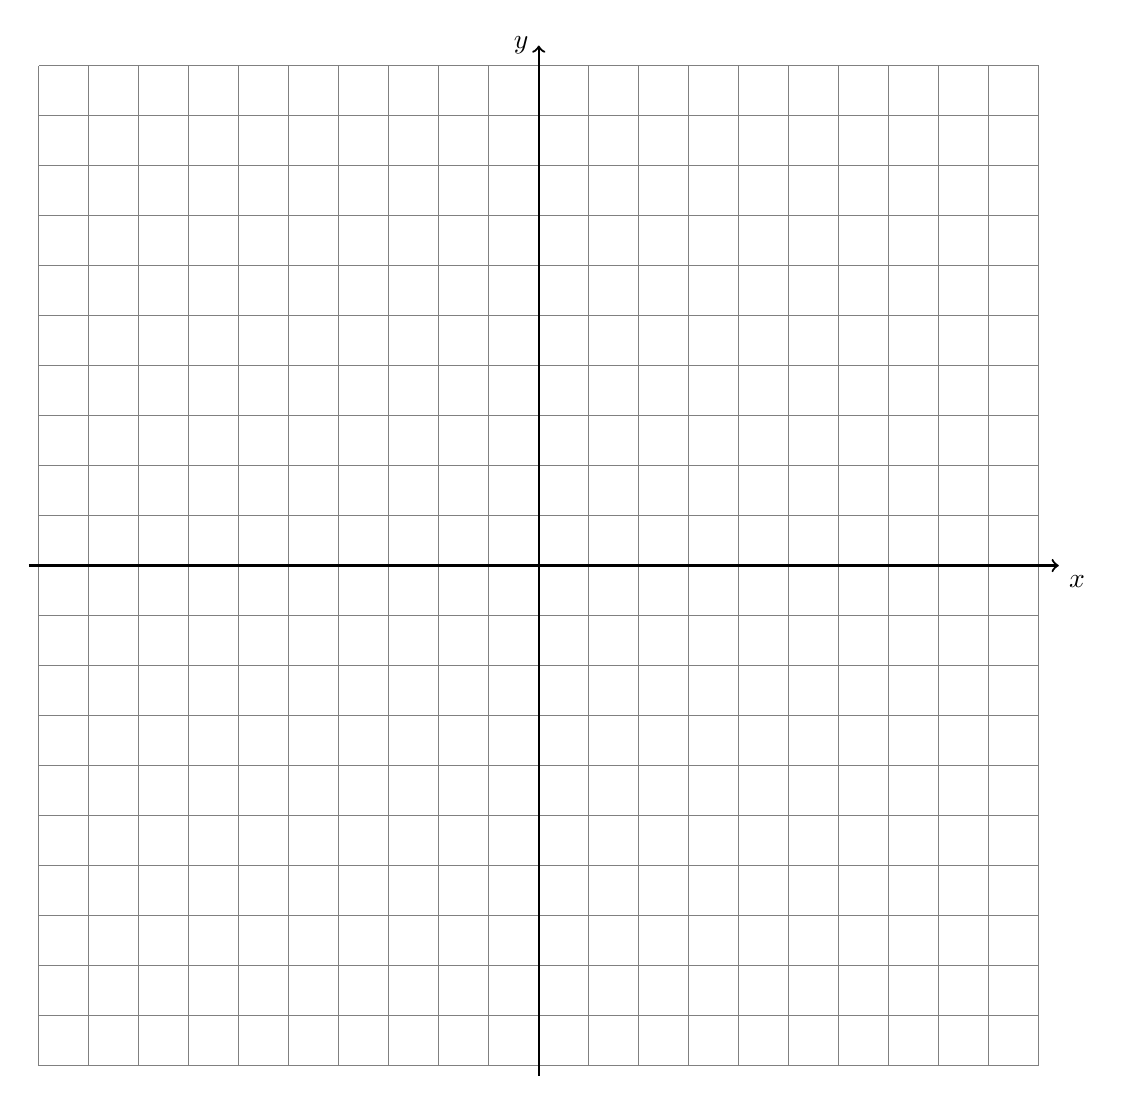
\begin{tikzpicture}[scale=.635]
          \draw [help lines] (-10,-10) grid (10,10);
          \draw [thick, ->] (-10.2,0) -- (10.4,0) node [below right] {$x$};
          \draw [thick, ->] (0,-10.2)--(0,10.4) node [left] {$y$};
        \end{tikzpicture}
        \end{center}
\newpage

    \item Graph the two lines after filling in the values in the blanks.\\[0.5cm]


    \begin{multicols}{2}
      $y= x -3$ \\
      $x+y = 1 $
    \end{multicols}
    \begin{multicols}{2}
      \raggedcolumns
      \begin{enumerate}
        \item $y$-intercept $b= \rule{2cm}{0.15mm}$ \\[0.5cm]
        \item Slope \hspace{0.7cm} $m= \rule{2cm}{0.15mm}$\\[0.5cm]
      \end{enumerate}
      \begin{enumerate}
        \item $y$-intercept $b= \rule{2cm}{0.15mm}$ \\[0.5cm]
        \item Slope \hspace{0.7cm} $m= \rule{2cm}{0.15mm}$\\[0.5cm]
      \end{enumerate}
    \end{multicols}

    Label both lines and the solution to the system, the intersection, as a coordinate pair. (3 points) Use pencil for graph (1 point)\\

    \begin{center} %4 quadrant regents grid w T-Chart
    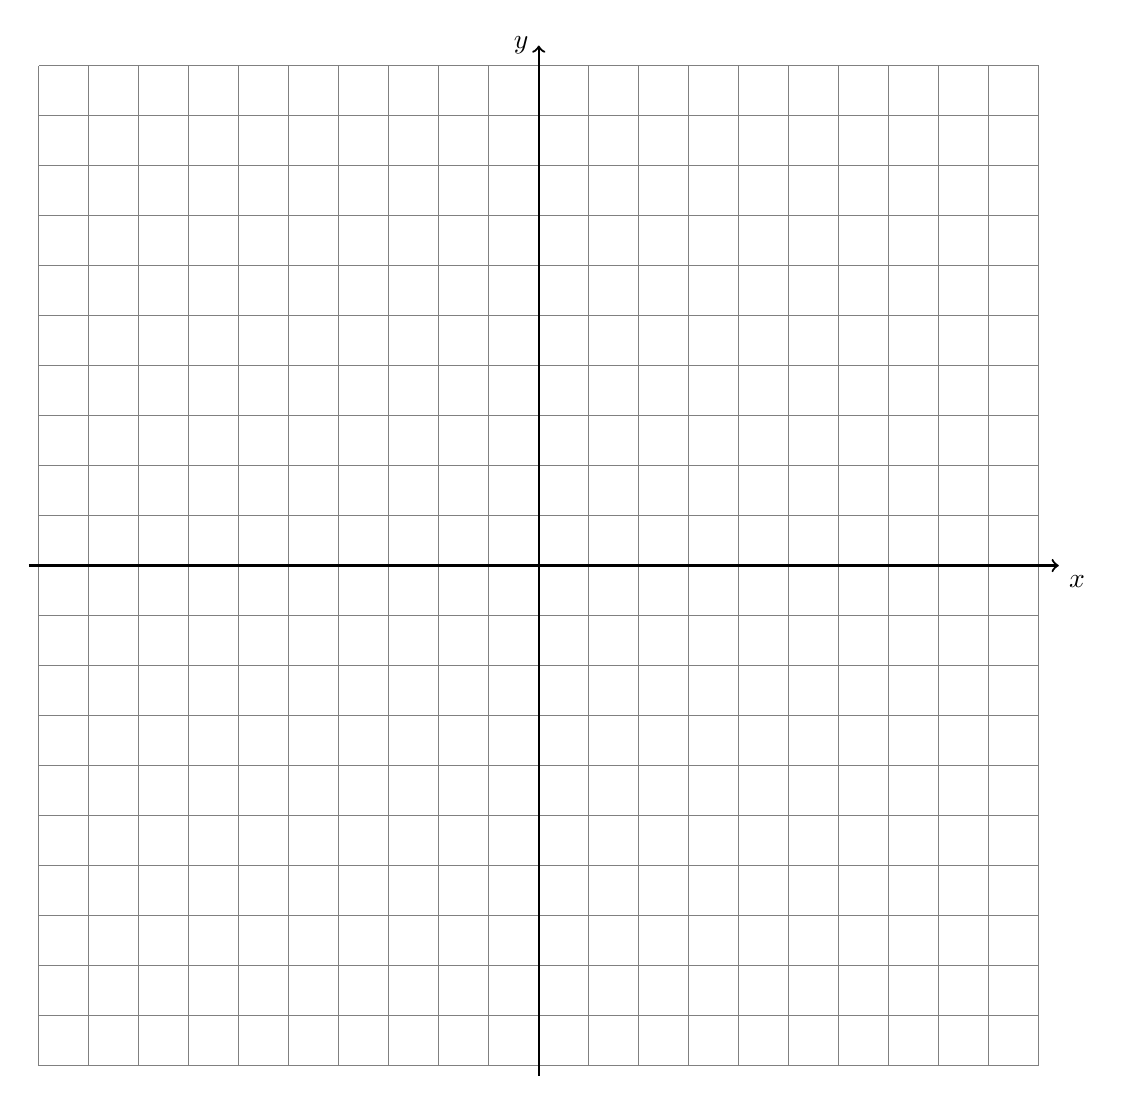
\begin{tikzpicture}[scale=.635]
      \draw [help lines] (-10,-10) grid (10,10);
      \draw [thick, ->] (-10.2,0) -- (10.4,0) node [below right] {$x$};
      \draw [thick, ->] (0,-10.2)--(0,10.4) node [left] {$y$};
    \end{tikzpicture}
    \end{center}

\end{enumerate}

\end{document}

  % problem 35 June 2018
  \item On the set of axes below, graph the following system of inequalities:
    \[2y+3x \leq 14 \]
    \[4x-y < 2\]

    10 by 10 grid

    Determine if the point $(1,2)$ is in the solution set. Explain your answer.

      In the following two problems, solve for the value of $x$.
      \begin{multicols}{2}
      \item   $11=2x+x-1$ \vspace{3cm}
      \item   $\frac{1}{3}(6-3x)=11$ %\vspace{3cm}
      \end{multicols}


    \subsubsection*{Simplify each expression (``Collect like terms")}
      \item $x^2-3x -4 +2x^2+2x+4$ \vspace{1.5cm}
      \item $5(a^2-3a +1) -2(a^2+2a-3)$ \vspace{3cm}
